\documentclass[letterpaper, 10 pt, conference]{ieeeconf}  % Comment this line out if you need a4paper

%\documentclass[a4paper, 10pt, conference]{ieeeconf}      % Use this line for a4 paper

\IEEEoverridecommandlockouts                              % This command is only needed if 
                                                          % you want to use the \thanks command

\overrideIEEEmargins                                      % Needed to meet printer requirements.

% The following packages can be found on http:\\www.ctan.org
\usepackage{graphics} % for pdf, bitmapped graphics files
%\usepackage{graphicx}
\usepackage[dvipdfmx]{graphicx}
\usepackage[dvipdfmx]{color}
\usepackage{epsfig} % for postscript graphics files
\usepackage{mathptmx} % assumes new font selection scheme installed
\usepackage{times} % assumes new font selection scheme installed
\usepackage{amsmath} % assumes amsmath package installed
\usepackage{amssymb}  % assumes amsmath package installed
\usepackage{multicol}
\usepackage{multirow}
\usepackage{url}
\usepackage{caption}
\usepackage[ruled,vlined]{algorithm2e}
%\include{pythonlisting}
\usepackage{algpseudocode}
\usepackage[dvipsnames]{xcolor}
\usepackage{cite}

\setlength\textfloatsep{5pt}

\title{\LARGE \bf
Time-Based Current Source (TBCS): A Highly-Digital Robust Current Generator for Switched Capacitor Circuits
}

\author{Kentaro Yoshioka% <-this % stops a space
%\thanks{*This work was not supported by any organization}% <-this % stops a space
\thanks{
        {\tt\small yoshioka@elec.keio.ac.jp}}
}

\begin{document}

\maketitle
\thispagestyle{empty}
\pagestyle{empty}

%%%%%%%%%%%%%%%%%%%%%%%%%%%%%%%%%%%%%%%%%%%%%%%%%%%%%%%%%%%%%%%%%%%%%%%%%%%%%%%%
\begin{abstract}
従来電流源は抵抗絶対値に生成電流が左右されるためばらつきに弱く生成する電流量のばらつきが大きいという課題があった。このようなばらつき下ではオペアンプの設計マージンが増大してしまい、システム消費電力が増大する。

そこで微細CMOSにおけるスイッチドキャパシタ回路に好適な基準電流源回路であるTime-Based Current Source (TBCS)を提案する。A delay-locked-loop (DLL) is constructed to lock the current-starved inverter with the sample clock of the ADC, and the settled current value is directly used as the reference current.
CSDの遅延は電流と負荷容量で決定されるため、遅延ロックした際の電流値はPVTに依らない値であるためロバストな基準電流源を構築できる。TBCSはほぼインバータセルと簡潔なデジタル回路で実現でき、微細化プロセスほど低コストとなる。またTBCSのユニークな点として負荷容量のばらつき応じ生成電流を変動させるが、これはスイッチドキャパシタ回路のオペアンプ特性を補償する特徴を持つ。

28nm CMOSで試作したTBCSは$1200um^2$と非常に小さい面積を達成した。またバンドギャップレファレンスに対し幅広いPVTばらつきにおいて電流変動を半分以下に抑えられることをシミュレーションで確認した。

\end{abstract}

%%%%%%%%%%%%%%%%%%%%%%%%%%%%%%%%%%%%%%%%%%%%%%%%%%%%%%%%%%%%%%%%%%%%%%%%%%%%%%%%
\section{Introduction}

Switched-capacitor (SC) circuits are the fundamental building blocks of high-precision, high-speed ADCs (e.g. pipelined ADCs and pipeline-SAR ADCs), which are critical circuit components to realize 5G and beyond 5G wireless-communication circuits \cite{5g1, 5g2, ali201414, ali202012, lagos2018single, hung2020calibration}. Among those, a reference current source is an important circuit that determines the operational amplifier (opamp) characteristics. Especially for high-speed SC circuits, the speed of the opamp is one of the most critical design parameters and must be carefully designed. However, while the PVT variation effects of the reference current source contribute significantly to the switched-capacitor circuit performance, the reference current source design itself has not received much attention in the literature.

There are two main design approaches for reference current sources: beta-multiplier or voltage-current conversion. Beta-multiplier, which generates a current in a self-bias fashion, exploits the complementary temperature characteristics of resistors and transistors to cancel the temperature dependence \cite{azcona2014precision, osipov2016temperature}. In the voltage-current conversion approach, a resistor performs voltage-current conversion utilizing a reference voltage generated by a robust bandgap reference (BGR) voltage source, which is highly robust to PVT variations\cite{banba1999cmos, ueno2009300, ueno20101}. On the other hand, the generated current is affected by the absolute resistance value in these methods. Since the current source for high-speed SC circuits requires currents in the order of several tens of uA, a poly-resistance device is typically used. However, during mass production, such resistors can vary by as much as $\pm40\%$ due to manufacturing variations, and the drift directly affects the generated current.

Therefore, a common practice is to calibrate such resistance variation at the time of shipping or allow it as a design margin. However, the former increases analog test costs, while the latter worsens the system power consumption, area, and yield due to the opamp overdesign. Some researches focus on replacing the resistors with transistors \cite{hirose2010nano, hirose2010cmos, osaki20131, choi201423pw}. However, its circuit area is largely due to the importance of analog characteristics. It may be challenging to reduce the cost even with scaled CMOS processes.

In this paper, we propose a time-based current source (TBCS) to realize a highly digital and low-cost current source \cite{yoshioka201728}. A delay-locked-loop (DLL) locks the current-starved delay-line (CSD) delay to the ADC sampling clock, and the locked current value is directly exploited as the reference current. 
Since the delay of the CSD is determined by the given current and load capacitance, a robust current source can be constructed; the current value when the delay is locked is decoupled from the transistor and resistor PVT variations.
Interestingly, while TBCS current varies with the variation of load capacitance, this characteristic compensates for the opamp characteristics of the SC. 
When the load capacitance increases, TBCS increases the current to keep the delay constant, which helps the opamp to drive the increased load capacitance and maintains the speed.
Moreover, the TBCS can be composed almost entirely of inverter cells and digital circuits and is highly process-scalable. The prototype circuit was fabricated with 28nm CMOS and occupied an area of only $1200um^2$.

In extension to ref.\cite{yoshioka201728, yoshioka2019digital}, this paper adds extensive analysis of TBCS. Specifically, we make the following contributions. 1) In-depth discussion of TBCS principles and circuit implications 2) Analyze the characteristics of opamp when incorporated with TBCS through detailed simulations, and confirm that TBCS compensates for the opamp speed. 
This paper is organized as follows: Section 2 describes the previous studies and their challenges. Section 3 explains the principle of TBCS and Section 4 discusses the circuit implementation of TBCS. Finally, Section 5 reports the simulation results and analysis.

%%%%%%%%%%%%%%%%%%%%%%%%%%%%%%%%%%%%%%%%%%%%%%%%%%%%%%%%%%%%%
\section{Related researches}
\begin{figure}[!]
\centering
 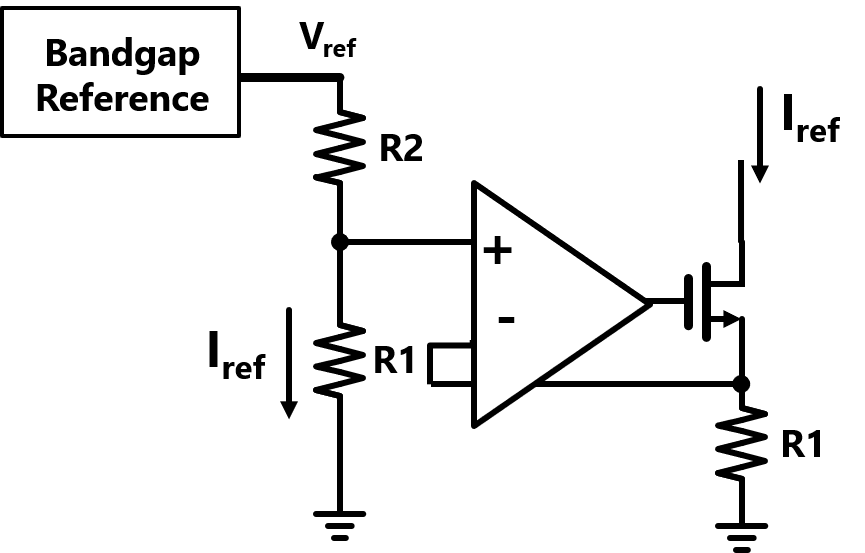
\includegraphics[width=0.5\textwidth]{figs/fig1.png}
  \caption{電圧-電流変換を用いたバンドギャップレファレンス型電流源}
\label{bandgap}
\end{figure}

\begin{figure*}[!]
\centering
 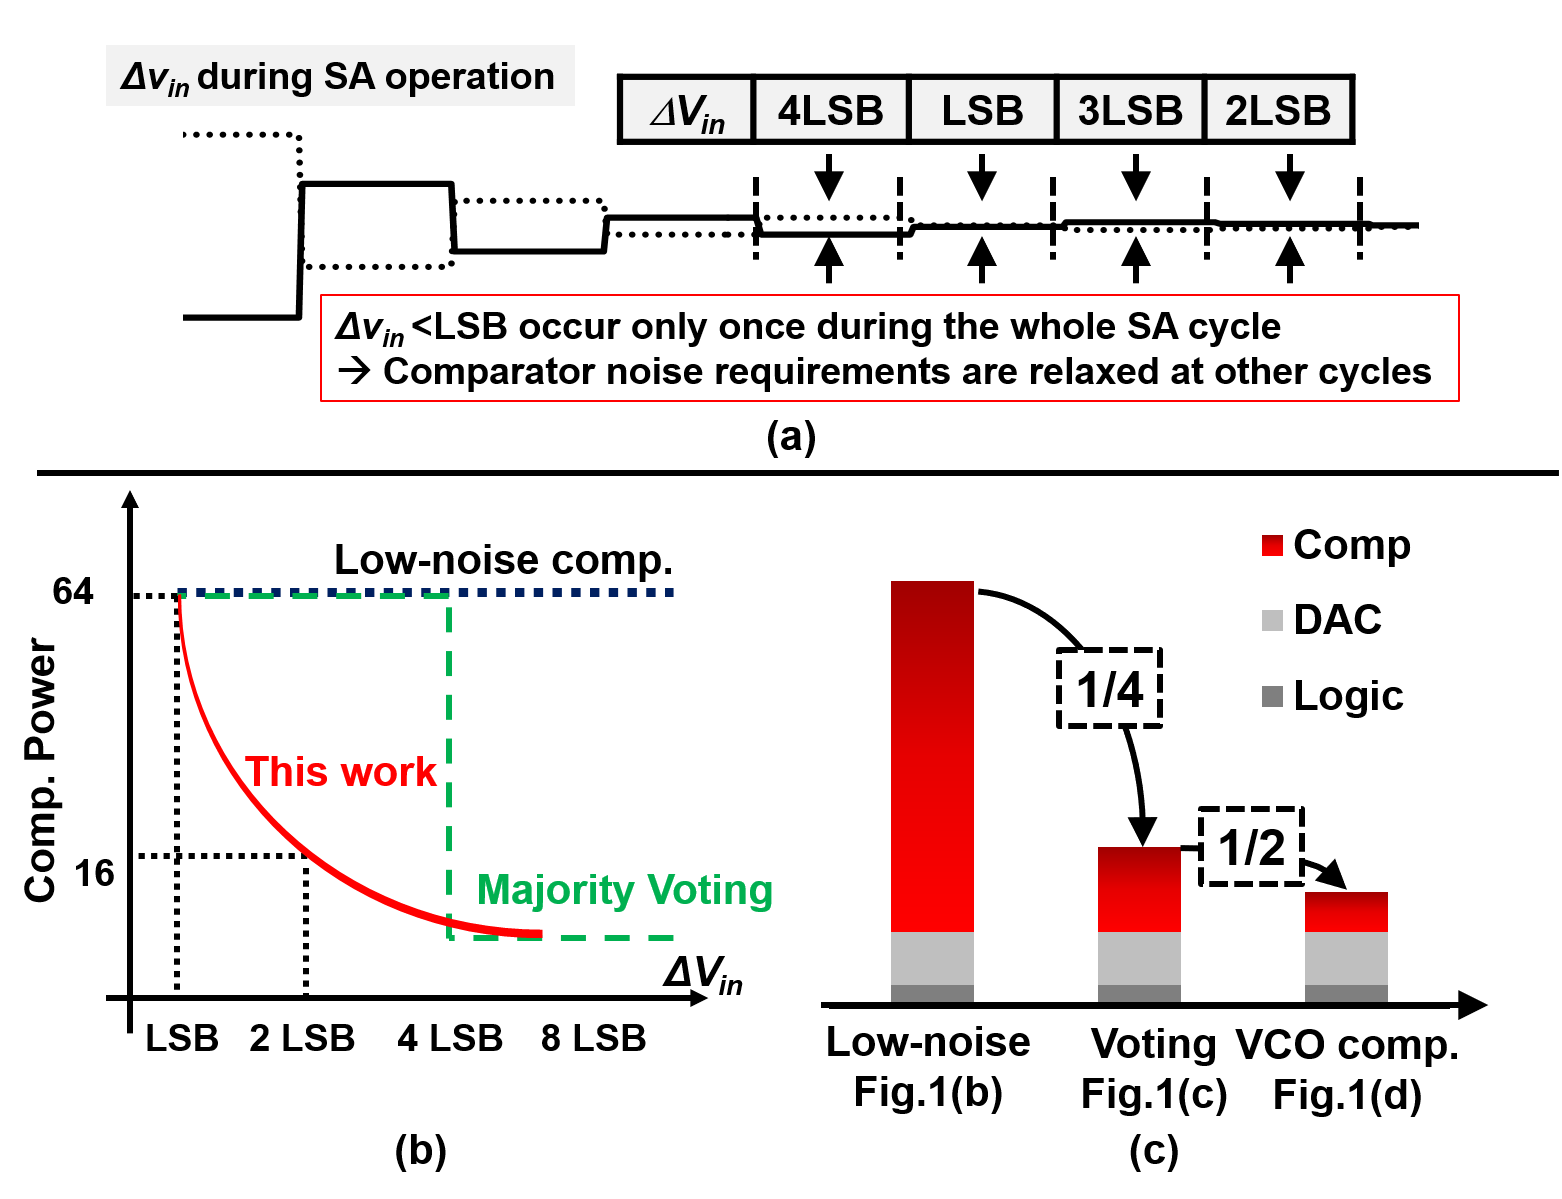
\includegraphics[width=0.9\textwidth]{figs/fig2.png}
  \caption{TBCSのブロック回路図。Current starved delay chainの遅延をCLKの半周期にロックするよう電流を制御する。遅延をロックした際の電流値は容量負荷に応じた値となりPVTばらつきに対して頑強であり、ロバストな電流源を実現できる。}
  \label{fig2}
\end{figure*}


\textbf{Bandgap reference} The BGR is widely used as a current source as shown in Fig.\ref{bandgap}. The BGR generates a robust reference voltage $V_{ref}$ and the reference current $I_{ref}$ is generated by voltage-current conversion as:
\begin{eqnarray}
    \centering
    I_{ref} = \frac{V_{ref}}{R_1 + R_2}
    \label{sar13b}
\end{eqnarray}
The BGR can generate a constant voltage without being affected by environmental variations (temperature, transistor threshold, supply voltage, etc.; hereafter referred to as PVT variation). On the other hand, the resistance values R1 and R2 suffer greatly from manufacturing variations, where the resistance values can vary by up to $\pm 40\%$ in the case of poly-resistors. Therefore, for example, when $I_{ref}$=20uA is targeted, we must expect the max-min current values to be 32uA and 12uA, respectively. Such variations increase the opamp design margin and impacts system power consumption.

\textbf{Adaptive current references} Current sources capable of PVT variations are important for analog products and much research has been undergone. Ref.\cite{chuanyang,ron} utilizes a replica opamp and a capacitive load and by directly monitoring the slew rate of the opamp, the current reference is configured to satisfy the target slew rate regardless of PVT variations.
While this method can realize a PVT adaptive current source, the overhead is that a replica opamp is required and significant power and area must be consumed. On the other hand, TBCS can realize a PVT-robust current source using mostly-digital circuits without analog components; the overhead is small.

\textbf{Analog circuit calibration techniques using time information} Ref.\cite{zhu} uses the time information of the reference clock to calibrate analog circuit characteristics. Specifically, the supply voltage is controlled to be a constant delay with a DLL and the basic idea is similar to TBCS. Additionally, ref.\cite{kapusta201314b,tomson} uses a DLL to control the delay of an asynchronous SAR clock to calibrate the DAC settling time.
However, these researches aim to calibrate the delay characteristics of the analog circuits. To the best of the author's knowledge, the proposed TBCS is the first approach to suppress the variation of a reference current source by using time information.

\section{Time based current source (TBCS)}
\subsection{TBCS fundamentals}
A simplified circuit block diagram of the TBCS is shown in Fig.\ref{fig2}. The TBCS requires only a  predetermined frequency clock ($CLK$), such as the sample clock of an ADC, and its components and operation are similar to a Delay-Locked-Loop circuit (DLL) \cite{ sidiropoulos1997semidigital, lee19942, razavi2018delay} The reference current source produces a reference current ($I_{ref}$) which is fed to the core circuitry (e.g. opamp). In TBCS, $I_{ref}$ is also given to the current-starved-delayline (CSD), and the CSD outputs $CLK_{CSD}$ which is a signal appending a delay to $CLK$. The appended delay in $CLK_{CSD}$ is expressed as $Nt_{DL}$, where the number of stages in the CSD is $N$ and the stage delay is $t_{DL}$. Note that the larger $I_{ref}$ is, the smaller $t_{DL}$ become and vice versa. Then, phase comparison is performed between $CLK_{CSD}$ and the inverted output of CLK ($CLK_B$). As a result, the reference current source is controlled so that the delay ($Nt_{DL}$) converge to the half-cycle time of CLK ($T_D$). Note that frequency references can be finely generated by crystal references, providing a precise reference independent of PVT variations.

また一般的なDLLではループフィルタ\cite{sidiropoulos1997semidigital}やデジタルフィルタ\cite{kim20172}を用いて精微な遅延を生成するが、本回路ではPVTに適応する電流源の設計が主目的であり遅延の精度は重要ではないためこのようなフィルタは使わない。

\begin{figure}[!]
\centering
 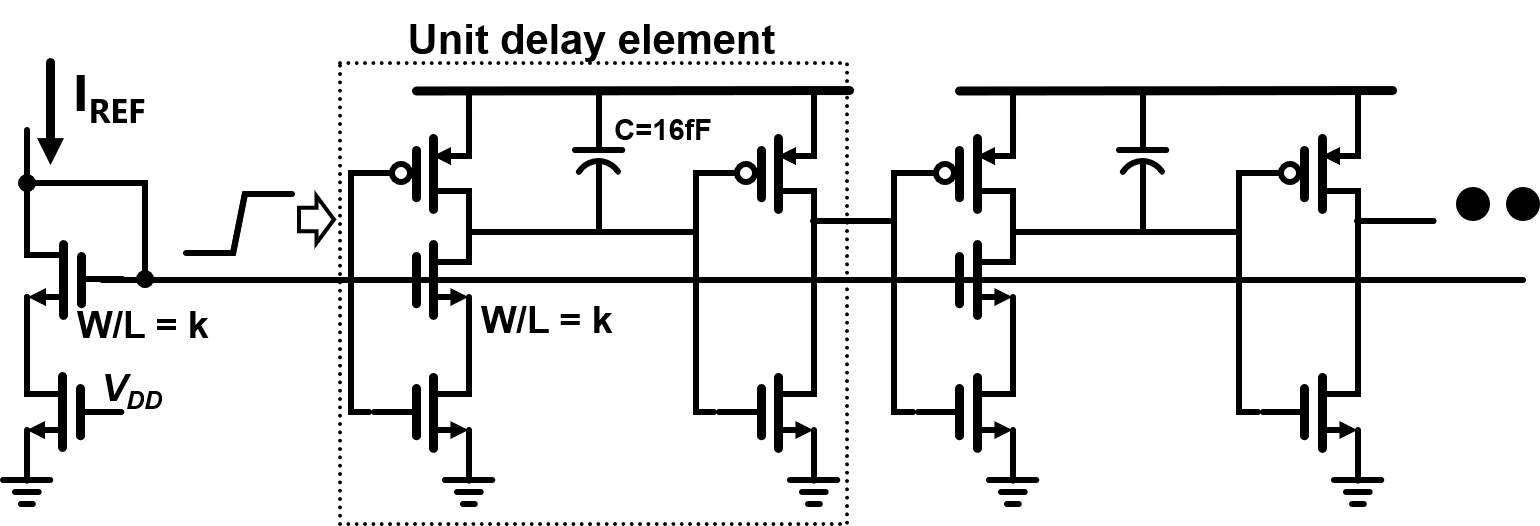
\includegraphics[width=0.5\textwidth]{figs/inv.png}
  \caption{Current starved delay chainの回路図}
\label{inv}
\end{figure}

By further studying the delay characteristics of the CSD, we show that the TBCS is capable of the robust current generation (Fig.\ref{fig2}(c)).
The circuit diagram of the CSD circuit is shown in Fig.\ref{inv}, consisting of a current-starved inverter(CSI)\cite{mroszczyk2014tunable} driving the capacitive load $C$ and the next-stage inverter. Based on the large-signal characteristics, the CSD delay $t_D$ can be expressed as: 
\begin{eqnarray}
    \centering
    t_D = \frac{V_{th}C}{I_{ref}}+t_{inv}
    \label{delay}
\end{eqnarray}
where $V_{th}$ and $t_{inv}$ is the on-threshold and the delay of the next-stage inverter, respectively.  Since the signal is fully propagated by the time the CSI current source enters the triode region, such effect can be neglected from analysis. In eq.\ref{delay}, if we assume that $t_{inv}$ and $V_th$ variation is sufficiently small, $t_D$ will be determined by $C$ and $I_{ref}$. 
Since TBCS converges $I_{ref}$ so that $t_{DL}$ to a predetermined value, thus after locking, $I_{ref}$ will become a value corresponding to the capacitance $C$. In advanced CMOS processes, capacitors are significantly less invariant to environmental variations such as voltage, temperature, and mismatch compared to resistors and transistors. Therefore, TBCS can achieve robust current generation independent of environmental variations with delay lock-based configuration.


From eq.(\ref{delay}), the TBCS variation factors are 1) load capacitance variation and 2) next-stage inverter delay + $V_{th}$ variation.
Since the delay of the next-stage inverter in (2) is one order of magnitude smaller than the CSI delay, its effect is small. On the other hand, the capacitance variation must be small for TBCS to be a robust current source. While metal-insulator-metal (MIM) capacitors have small local mismatches, it is not suitable for TBCS due to its large absolute capacitance variation. On the other hand, metal-oxide-metal (MOM) capacitors have a significantly smaller absolute capacitance variation, making it suitable for TBCS. Moreover, we will show that the current drifts due to capacitance variation can help to stabilize the opamp characteristics in the next section.

\subsection{PVT adaptive current generation characteristics}
\begin{figure}[!]
\centering
 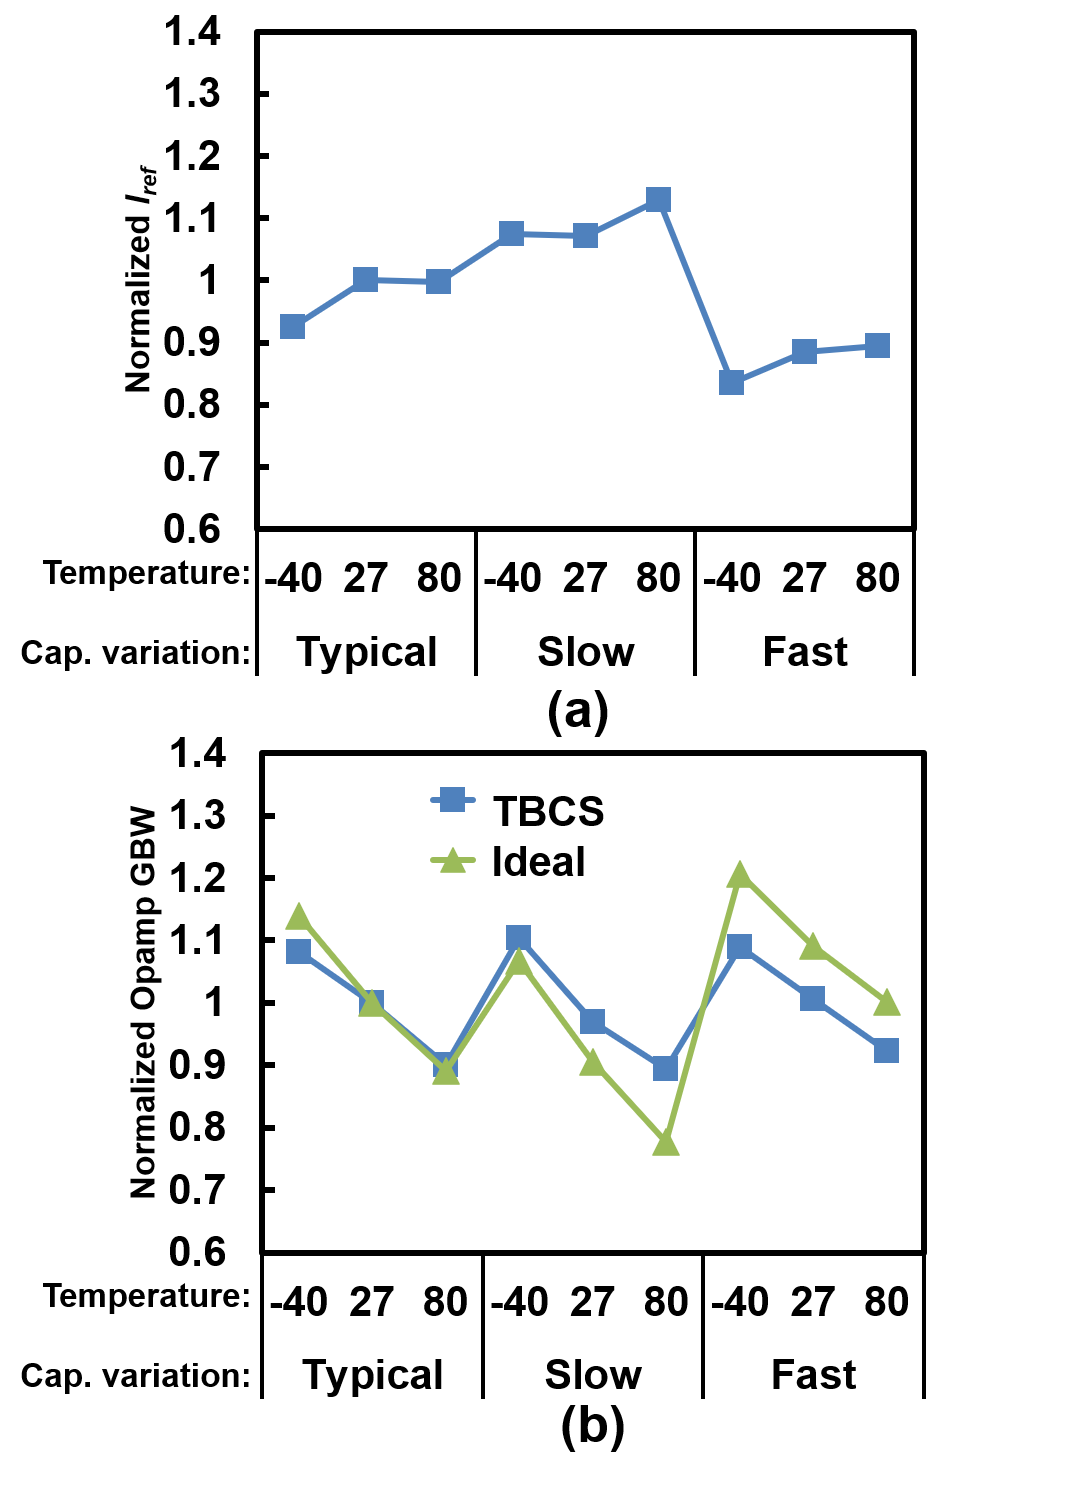
\includegraphics[width=0.5\textwidth]{figs/iref_var.png}
  \caption{(a)負荷容量が増大するばらつき条件におけるTBCSの生成電流のシミュレーション結果。(b)同ばらつき下においてTBCSと理想電流源でそれぞれバイアスしたオペアンプGBWの変動のシミュレーション結果}
\label{cvar}
\end{figure}

While the TBCS is decoupled from transistor and resistor variation, the capacitor variation causes current drifts since $T_{DL}$ is determined by the capacitor charging time. Interestingly, the current drift due to the capacitance variation militates to improve the opamp PVT tolerance.
From eq.(\ref{delay}), as $C$ increases, $I_{ref}$ will increase, and conversely, as $C$ decreases, $I_{ref}$ decreases. Such characteristic is undesirable from the viewpoint of a \textit{constant} current source. On the other hand, it is important to note that when such capacitance variation occurs, the load capacitance of the opamp increases/decrease as well. As the load capacitance increases, the gain-bandwidth (GBW) of the opamp degrades; however, the TBCS \textit{adaptively} increases the current to compensate for the degraded GBW. Thus, the TBCS will help to keep the opamp GBW constant through PVT variations.

To further analyze this effect, we perform extensive simulations. Fig.\ref{cvar}(a) and (b) show the generated TBCS current ($I_{ref}$) under capacitance variations and the variation of the opamp  GBW under the same variation, respectively. Here, a simple two-stage differential opamp (biased via TBCS) was utilized for simulations. In the "slow" conditions, the $I_{ref}$ increases by about 10-15\%, which compensates the opamp GBW degraded by the increased load capacitance. Interestingly, due to the adaptive current generation, TBCS can maintain opamp GBW constant through variations than an ideal current source. Under "fast" conditions, the $I_{ref}$ is reduced, but the effect on GBW is small because the opamp load is also reduced; TBCS operates to reduce power consumption while maintaining the required opamp GBW.

In general, mass-produced chips are designed to meet the critical performance (e.g. opamp GBW) even under the worst variations. Therefore, if we can supress GBW degradation under the worst condition, the design margin can be significantly reduced to improve the system power consumption. In Fig.\ref{cvar}(b), the GBW under the worst condition is improved by 13\% with TBCS over the ideal current source, proving that TBCS contributes to the design margin reduction.

\subsection{CLK入力周波数について}
本設計ではクロック周波数は80MHzが入力されると想定してCSDを設計した。無線機をアプリケーションとして考えているため他に動作周波数としては20MHz,40MHzが考えられるが、その場合TBCSの電流は最低値に張り付く。オペアンプは最低電流でもファンクションするように設計するのが一つの方法である。

また周波数を問わず一定電流を生成したいケースもあり、そのような場合に適応できる設計アイデアを示す。無線受信機用ADCのように使用するクロック周波数に整数倍の関係性がある場合、CSDを複数回発振させることで一定電流を生成可能である。入力クロックが設計周波数の1/4(20MHz)である場合、図xxのようにカウンタを用いてCSDを4回発振させることで80MHzに近い状態で電流源をロックさせ一定電流を生成できる。ただカウンタに入力周波数状態は与える必要があるのに注意したい。

%またCSDのM段目出力を用いて位相比較を行うようことでfractional周波数においても電流生成が可能である。カウンタを制御するための周波数情報は前もって入力する必要はあるが一般的にPLLはそのような情報を元に周波数を生成しているため情報を得るのは容易い。

\section{Circuit Implementations}
\subsection{Control circuit}
\begin{figure}[!]
\centering
 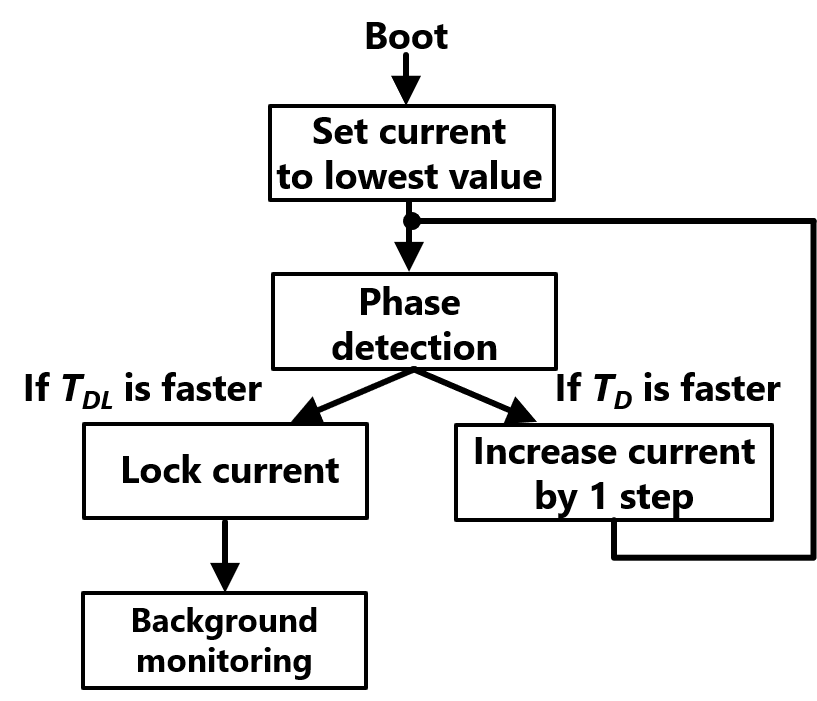
\includegraphics[width=0.5\textwidth]{figs/flowchart.png}
  \caption{TBCS制御のフローチャート}
\label{flow}
\end{figure}
Firstly, the basic control flow of TBCS is explained in detail using Fig.\ref{flow}. When the power is turned on, the current source is set to output the lowest $I_{ref}$. Then, the optimal current code is searched by increasing the code step by step. Since $I_{ref}$ is small at the beginning, $T_{DL}$ is prolonged and the phase detector judge that $T_D$ arrives early. Then, $I_{ref}$ is increased by one step. This procedure is repeated and once $T_{DL}$ arrives earlier, the current is "locked" and TBCS enters the background tracking mode.

Since this control method is a simple bang-bang control, maximum of $2^N$ cycles are required to converge ($N$ is the number of bits in the current source). For example, if we utilize successive approximation, we can achieve faster convergence. However, it may not be possible to track the environment drifts during the locking procedure (e.g. sharp voltage drifts).

\subsection{Phase detector}

\begin{figure}[!]
\centering
 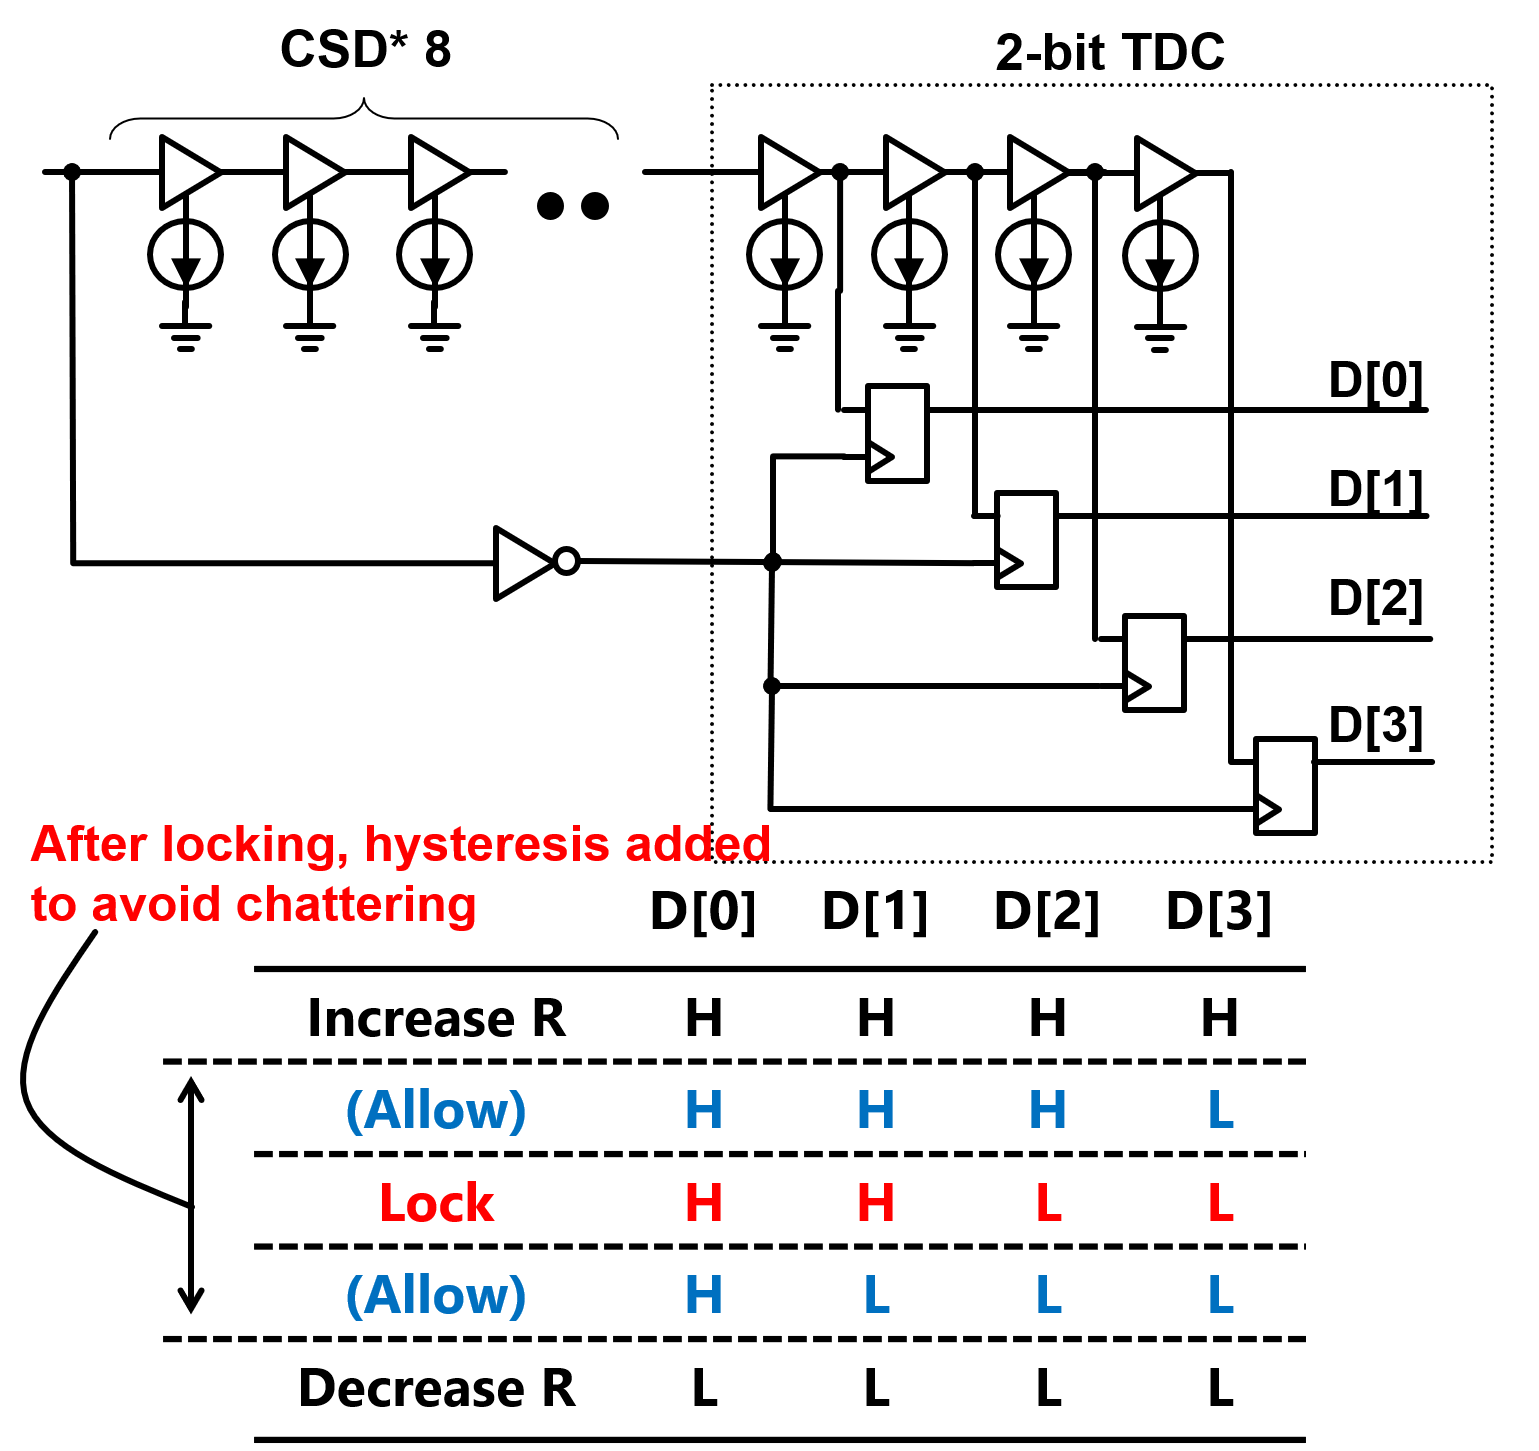
\includegraphics[width=0.5\textwidth]{figs/tdc.png}
  \caption{2-bit TDC回路とバックグラウンドモニタリング時の制御}
\label{tdc}
\end{figure}

\begin{figure}[!]
\centering
 
\includegraphics[width=0.5\textwidth]{figs/chattering.png}
  \caption{チャタリングが発生した際のタイミングチャート}
\label{chattering}
\end{figure}

Next, we will discuss the implementation of the phase detector. While an 1-bit TDC can be easily realized with a single flip-flop, there is a possibility of code flapping (chattering) which is illustrated in Fig.\ref{chattering}. If $I_{ref}$ is increased in the first phase cycle (code 14 to 15), the delay become smaller than $T_D$ in the next phase comparison. Thus, $I_{ref}$ is now reduced in response to the phase detector result (codes 15 to 14). Due to chattering which changes the current value every cycle, there is a risk of unwanted spurs in the SC circuit  While chattering can be prevented by fixing the control code after the current is locked, but TBCS will lose the ability to track PVT drifts.

In our design, we utilize a 2-bit TDC as the phase detector to prevent chattering and  provide PVT drift tracking (Fig.\ref{tdc}).
Once the current is locked, the TBCS enters the background monitoring mode to track long-term environmental variations.  As shown in the table of Fig.\ref{tdc}, the current code is not updated except when all the D[0:3] bits transitions to High or Low, which prevents chattering but can respond to long-term environmental changes. Note that before locking, only bit D[1] is used for control (identical to 1-bit TDC), and after locking, the full 2-bit output D[0:3] is utilized.

\subsection{R-DAC based current generator}
\begin{figure}[!]
\centering
 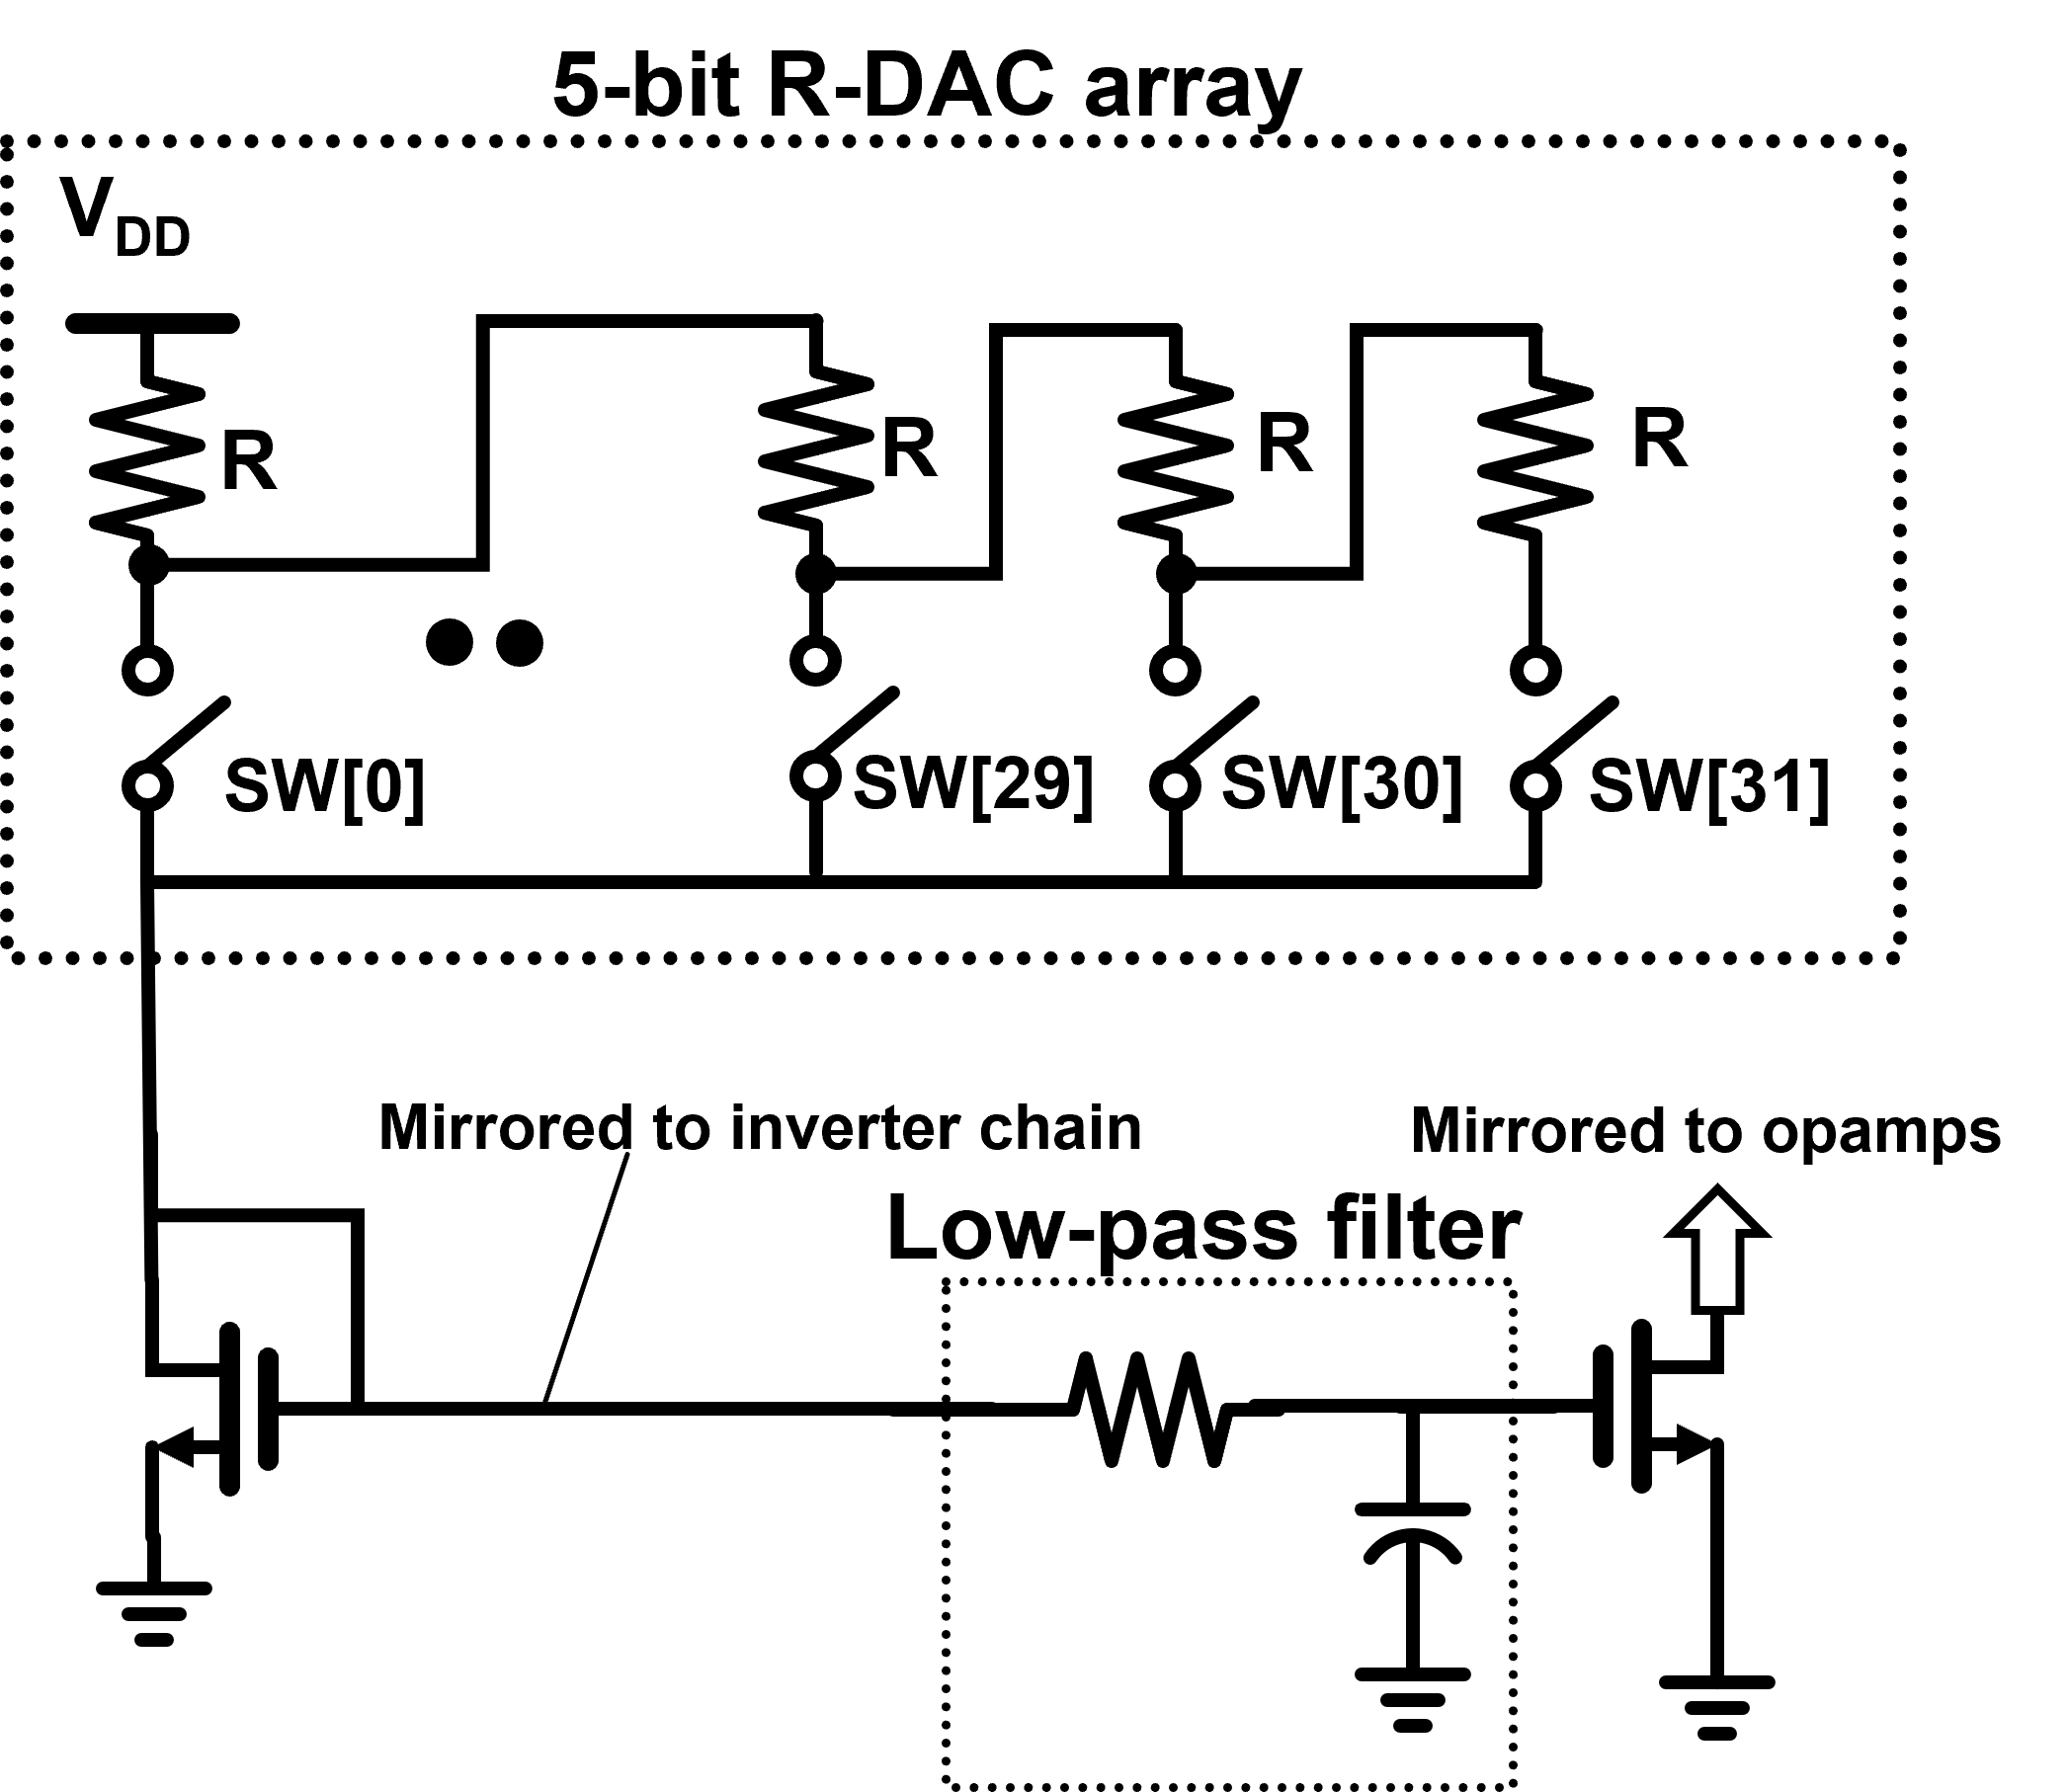
\includegraphics[width=0.5\textwidth]{figs/rdac.png}
  \caption{5-bit R-DACとローパスフィルタの回路図}
\label{rdac_sche}
\end{figure}

The circuit diagram of the R-DAC which constructs the variable reference current source is shown in Fig.\ref{rdac_sche}. The generated current $I_{ref}$ is decided by configuring the resistance value of the R-DAC as:
\begin{eqnarray}
    \centering
     I_{ref} = \frac{V_{DD}}{R_{NMOS}+R_{DAC}}
    \label{iref_eq}
\end{eqnarray}
The R-DAC is controlled by a one-hot digital code (SW[0:31]): when SW[31] is high, the resistance takes the maximum value of 32R and the lowest value R at SW[0]. In TBCS, the R-DAC design is the most critical factor. Specifically, the R-DAC must be designed to satisfy the following two points: (1) whether the accuracy of the generated current is sufficient and (2) whether the target current value can be generated even under PVT variations.

\begin{table}[]
\centering
 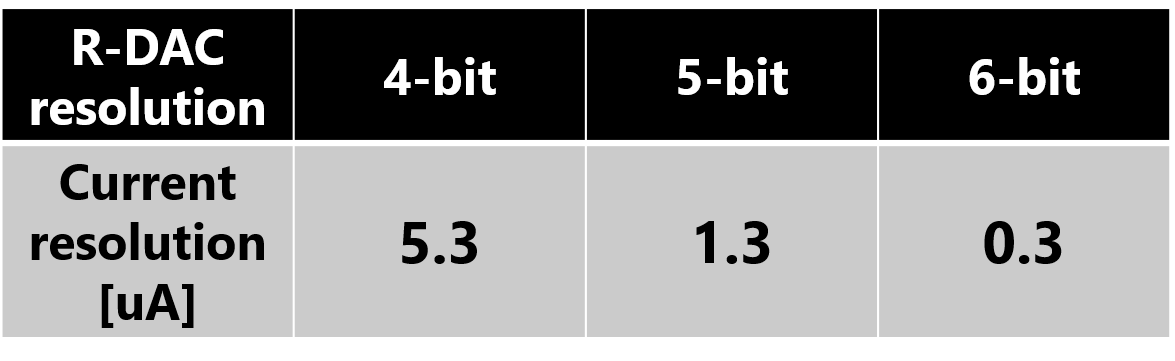
\includegraphics[width=0.4\textwidth]{figs/rdac_table.png}
  \caption{4, 5, 6-bit R-DACを用いた際のそれぞれにおける生成電流分解能. 単位抵抗は4kΩを使用。}
\label{rdac_table}
\end{table}

First of all, the R-DAC resolution directly couples to the generated current precision as shown in eq.(\ref{iref_eq}). Table \ref{rdac_table} summarizes the simulation result of the $I_{ref}$ resolution when the R-DAC resolution was varied from 4, 5 to 6 bits. In simulations, we adapt the current differential of the center code for simplicity. The 4-bit R-DAC had a step of 5uA, which is too large for our design. On the other hand, the 5-bit R-DAC had a step of 1.3uA, which is sufficient precision.

\begin{figure}[!]
\centering
 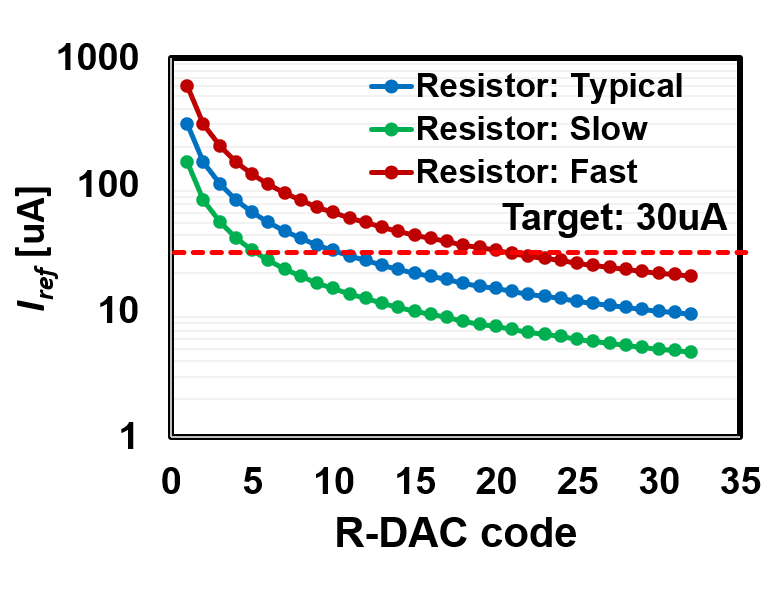
\includegraphics[width=0.5\textwidth]{figs/rdaccode.png}
  \caption{抵抗ばらつき下におけるR-DACコード対生成電流のシミュレーション結果}
\label{rdac_pvt}
\end{figure}

(2)に関しては抵抗のPVTばらつき下でも目標電流値にロックできるか確認する必要がある。図\ref{rdac_pvt}に抵抗のPVT におけるDACコードvs 生成電流をプロットした。今回目標とする30uAの電流生成はSlowからFast条件全てでカバーできることがわかる。もし抵抗ばらつきが大きくターゲットをカバーできないのならば、R-DAC分化能を増やすことで抵抗可変範囲を広く取る必要がある。

また図\ref{rdac_sche}に示すとおりTBCSは抵抗切替時に不要なスプリアスがオペアンプに伝搬してしまう可能性がある。そのような不要成分を取り除くため受動素子によりローパスフィルタを構成し、オペアンプへミラーするバイアスのスイッチング成分を除去している。

\subsection{Current starved delaylines}
\begin{figure}[!]
\centering
 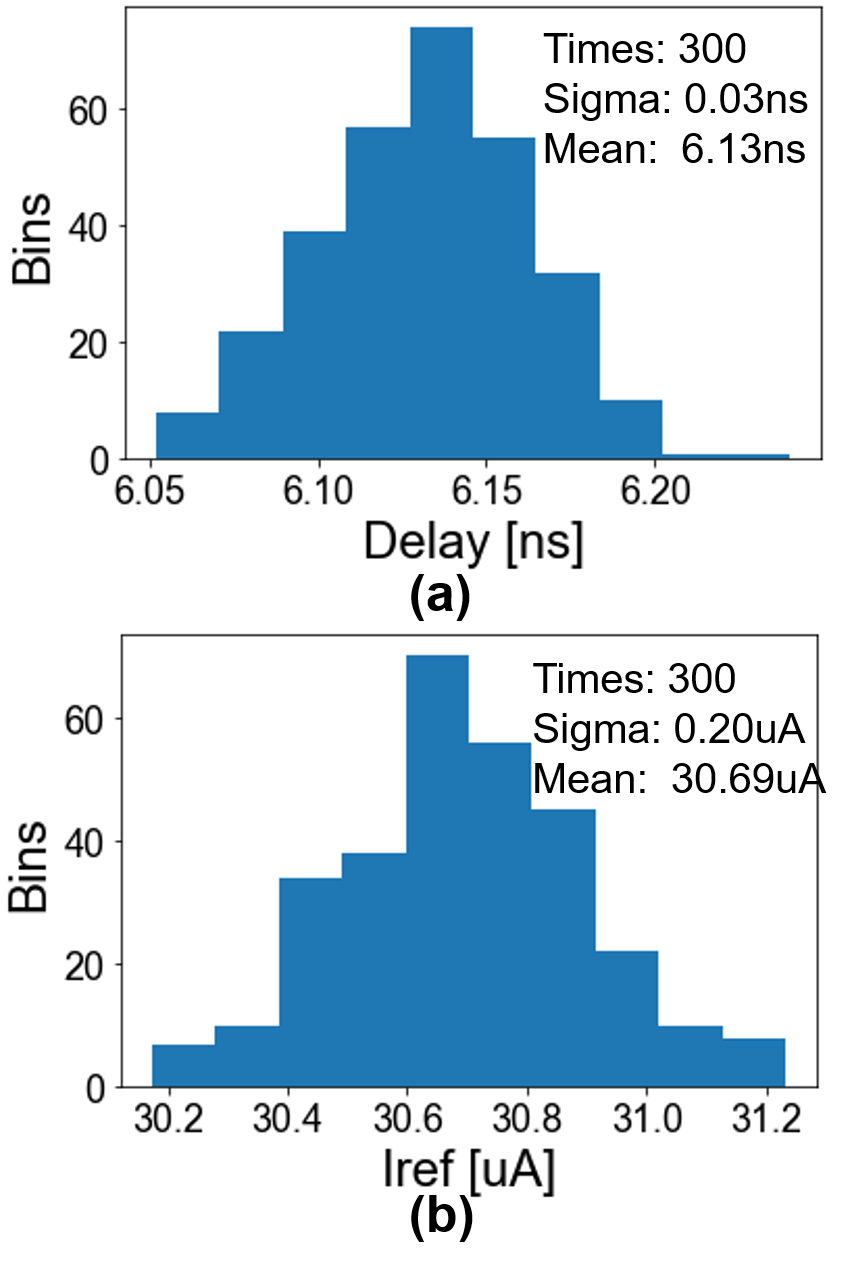
\includegraphics[width=0.35\textwidth]{figs/mc.png}
  \caption{(a) 
}
\label{monte}
\end{figure}

Finally, we describe the current starved delay-line (CSD) shown in Fig.\ref{inv}. While resistance mismatch affects $I{ref}$ in conventional current sources, the effect of resistance mismatch is small in TBCS due to the delay-locking feature. However, the CSD delay time variation has an adverse effect on $I{ref}$.
If we denote the delay mismatch of the single delayer as $var$, the overall variation of the $N$-stage CSD increases to $var \times \sqrt(N)$. However, since the signal component also become  $N$ times larger, the variation is mitigated to $\frac{1}{\sqrt(N)}$.

Fig.\ref{monte} shows the results of the Monte Carlo analysis. The overall delay variation is about $\sigma= 30 ps$ in this design, which is small enough compared to the TDC LSB step of 600 ps. As can be seen from the results of Fig.\ref{monte}(b), the effect of mismatch on $I_{ref}$ is small compared to the current resolution of 1.3uA. For a more accurate current generation, a finer TDC LSB will be required and the CSD variation may be reduced.
While jitter is also an important design factor in DLLs, the effect is small in TBCS. Since the jitter is sufficiently small compared to the total delay and TBCS uses hysteresis after locking, the jitter effect can be neglected.

\section{Measurement and simulation analysis}
\begin{figure}[!]
\centering
 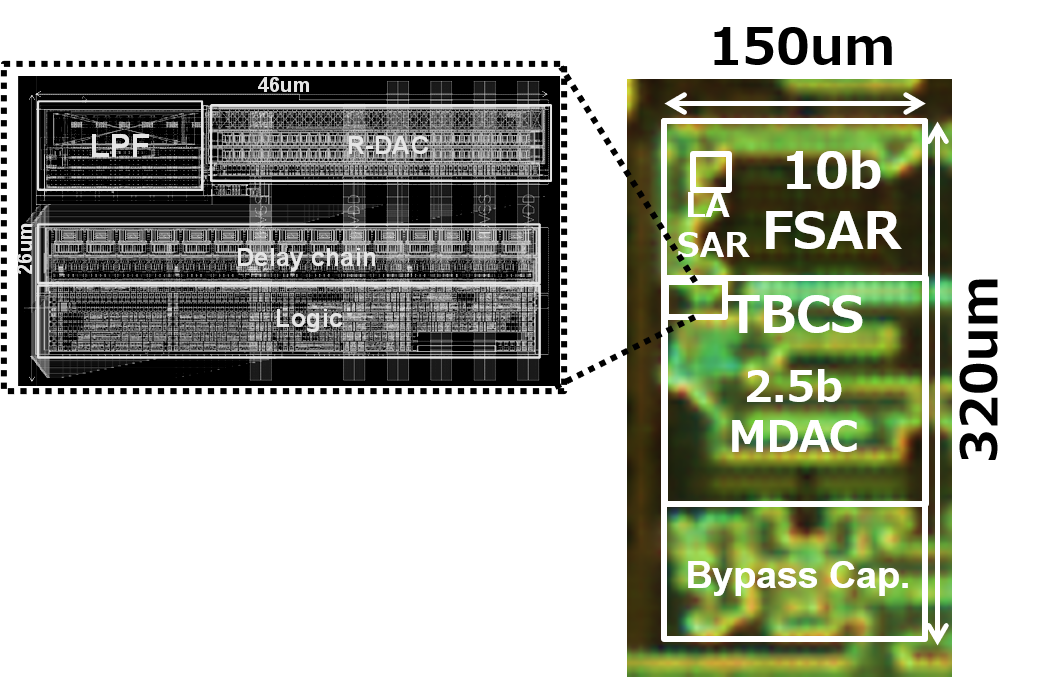
\includegraphics[width=0.5\textwidth]{figs/chip.png}
  \caption{チップ写真とレイアウト図、そしてパフォーマンスサマリー}
\label{chip}
\end{figure}

\begin{figure}[!]
\centering
 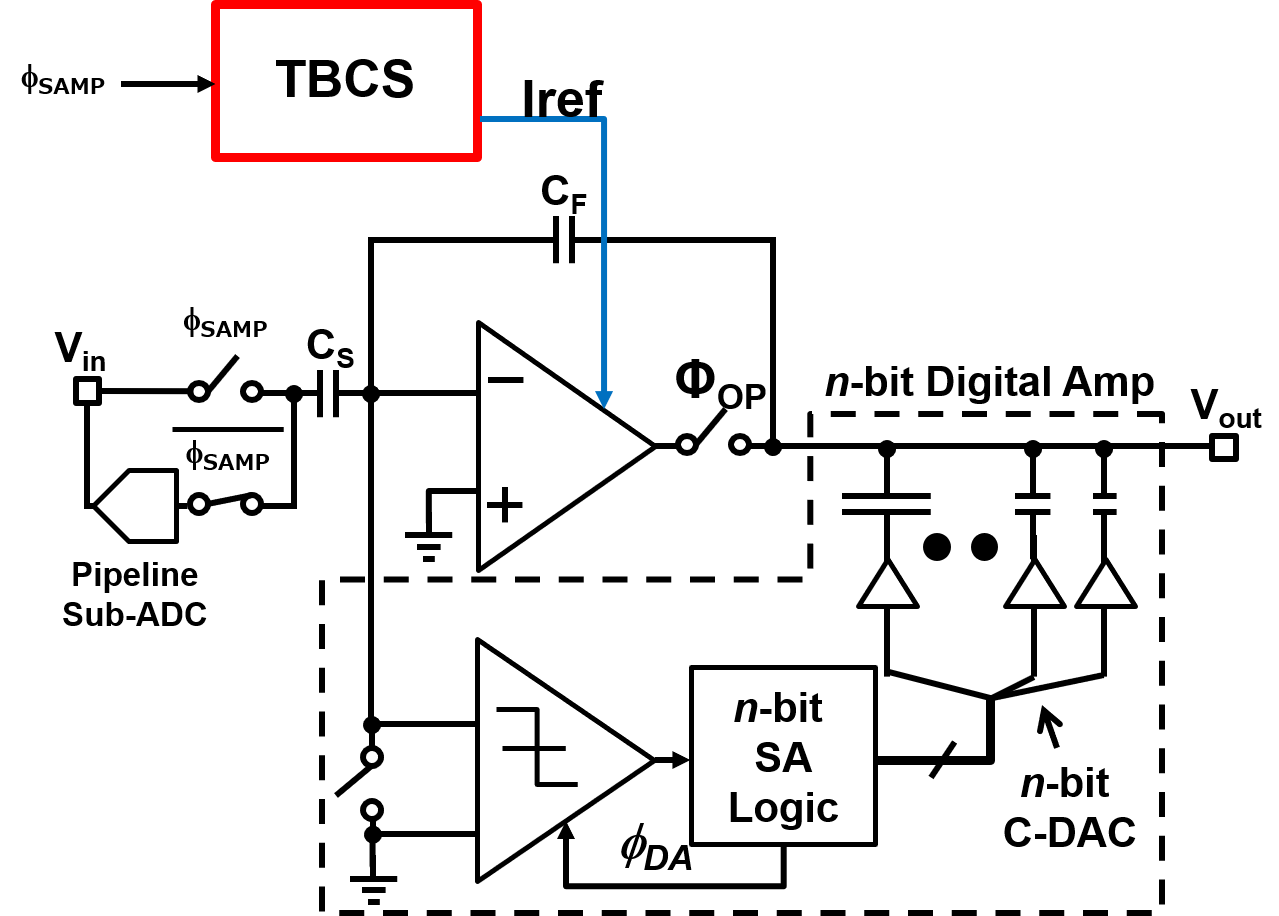
\includegraphics[width=0.5\textwidth]{figs/switchcap.png}
  \caption{試作チップのスイッチドキャパシタ回路図。}
\label{scap}
\end{figure}

\begin{figure}[!]
\centering
 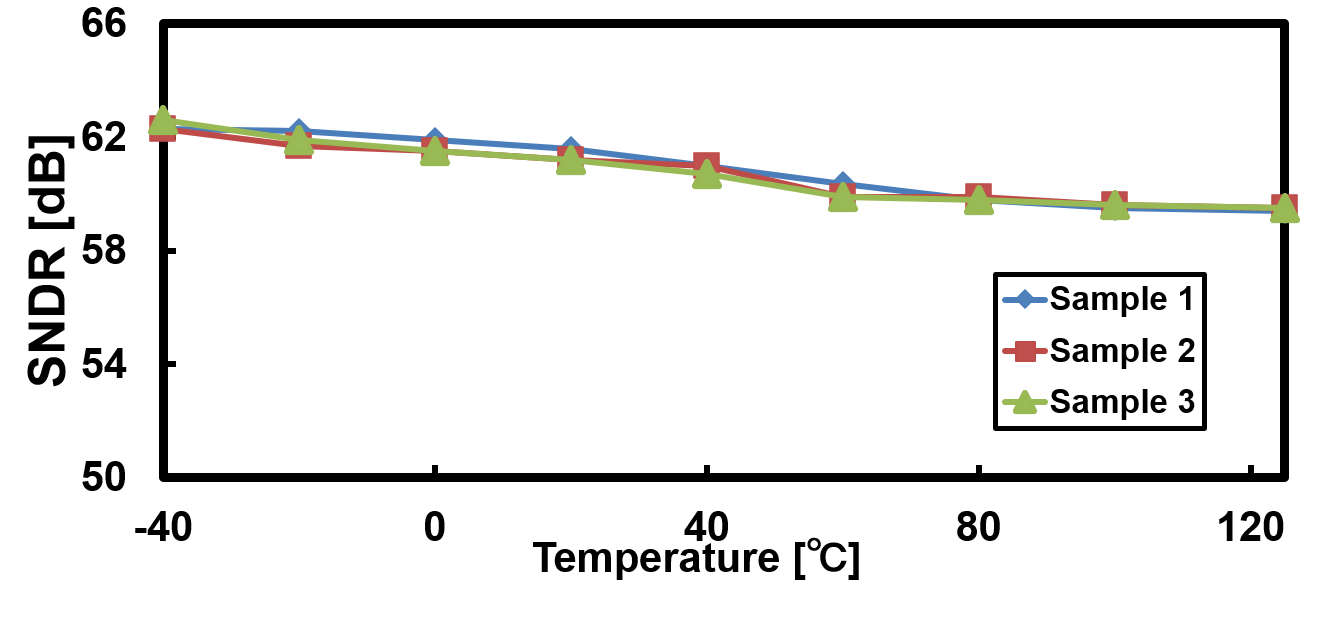
\includegraphics[width=0.5\textwidth]{figs/sndr.png}
  \caption{試作ADCのSNDR評価結果}
\label{sndr}
\end{figure}

\begin{figure}[!]
\centering
 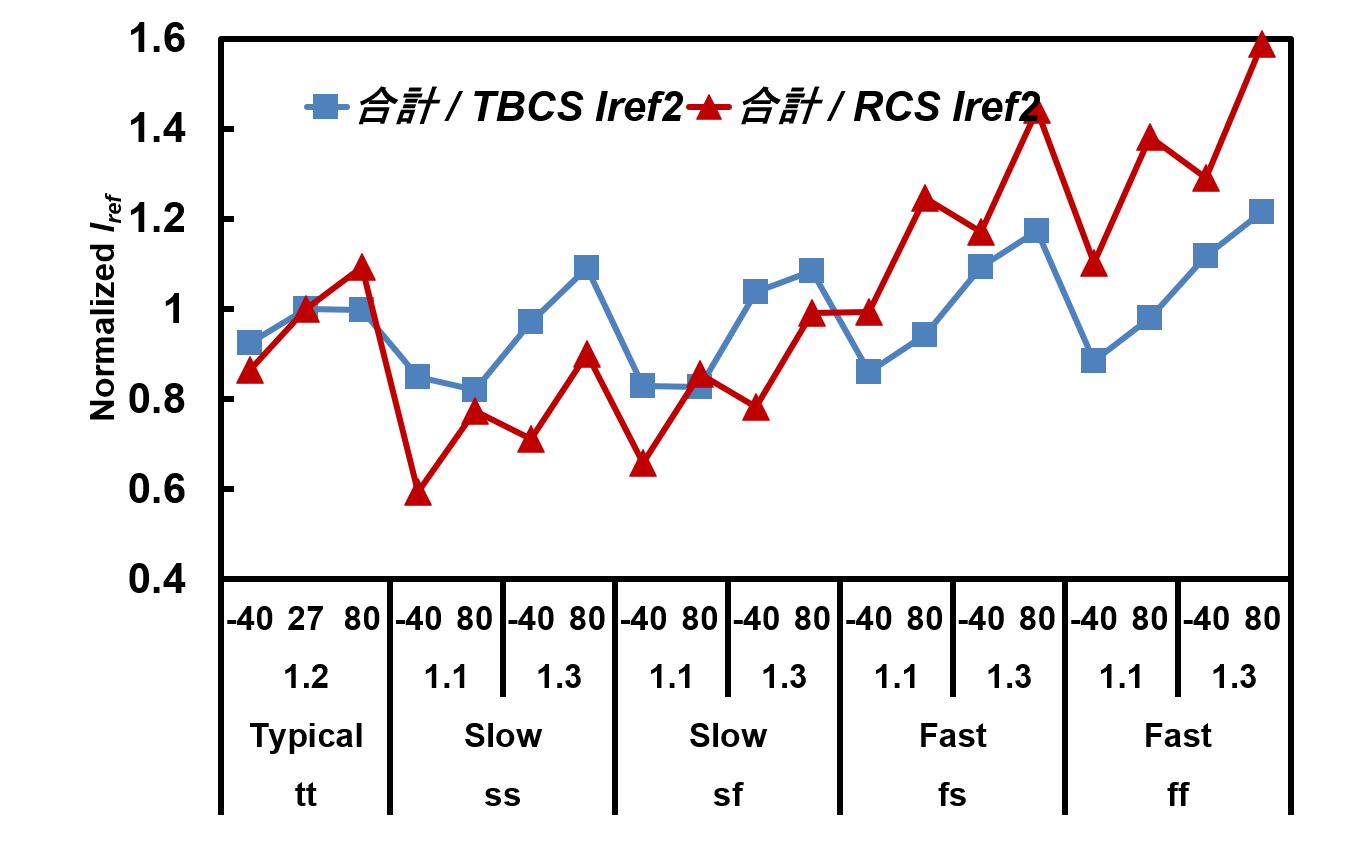
\includegraphics[width=0.5\textwidth]{figs/pvt.png}
  \caption{(a) 
}
\label{iref_pvt_both}
\end{figure}

\begin{figure}[!]
\centering
 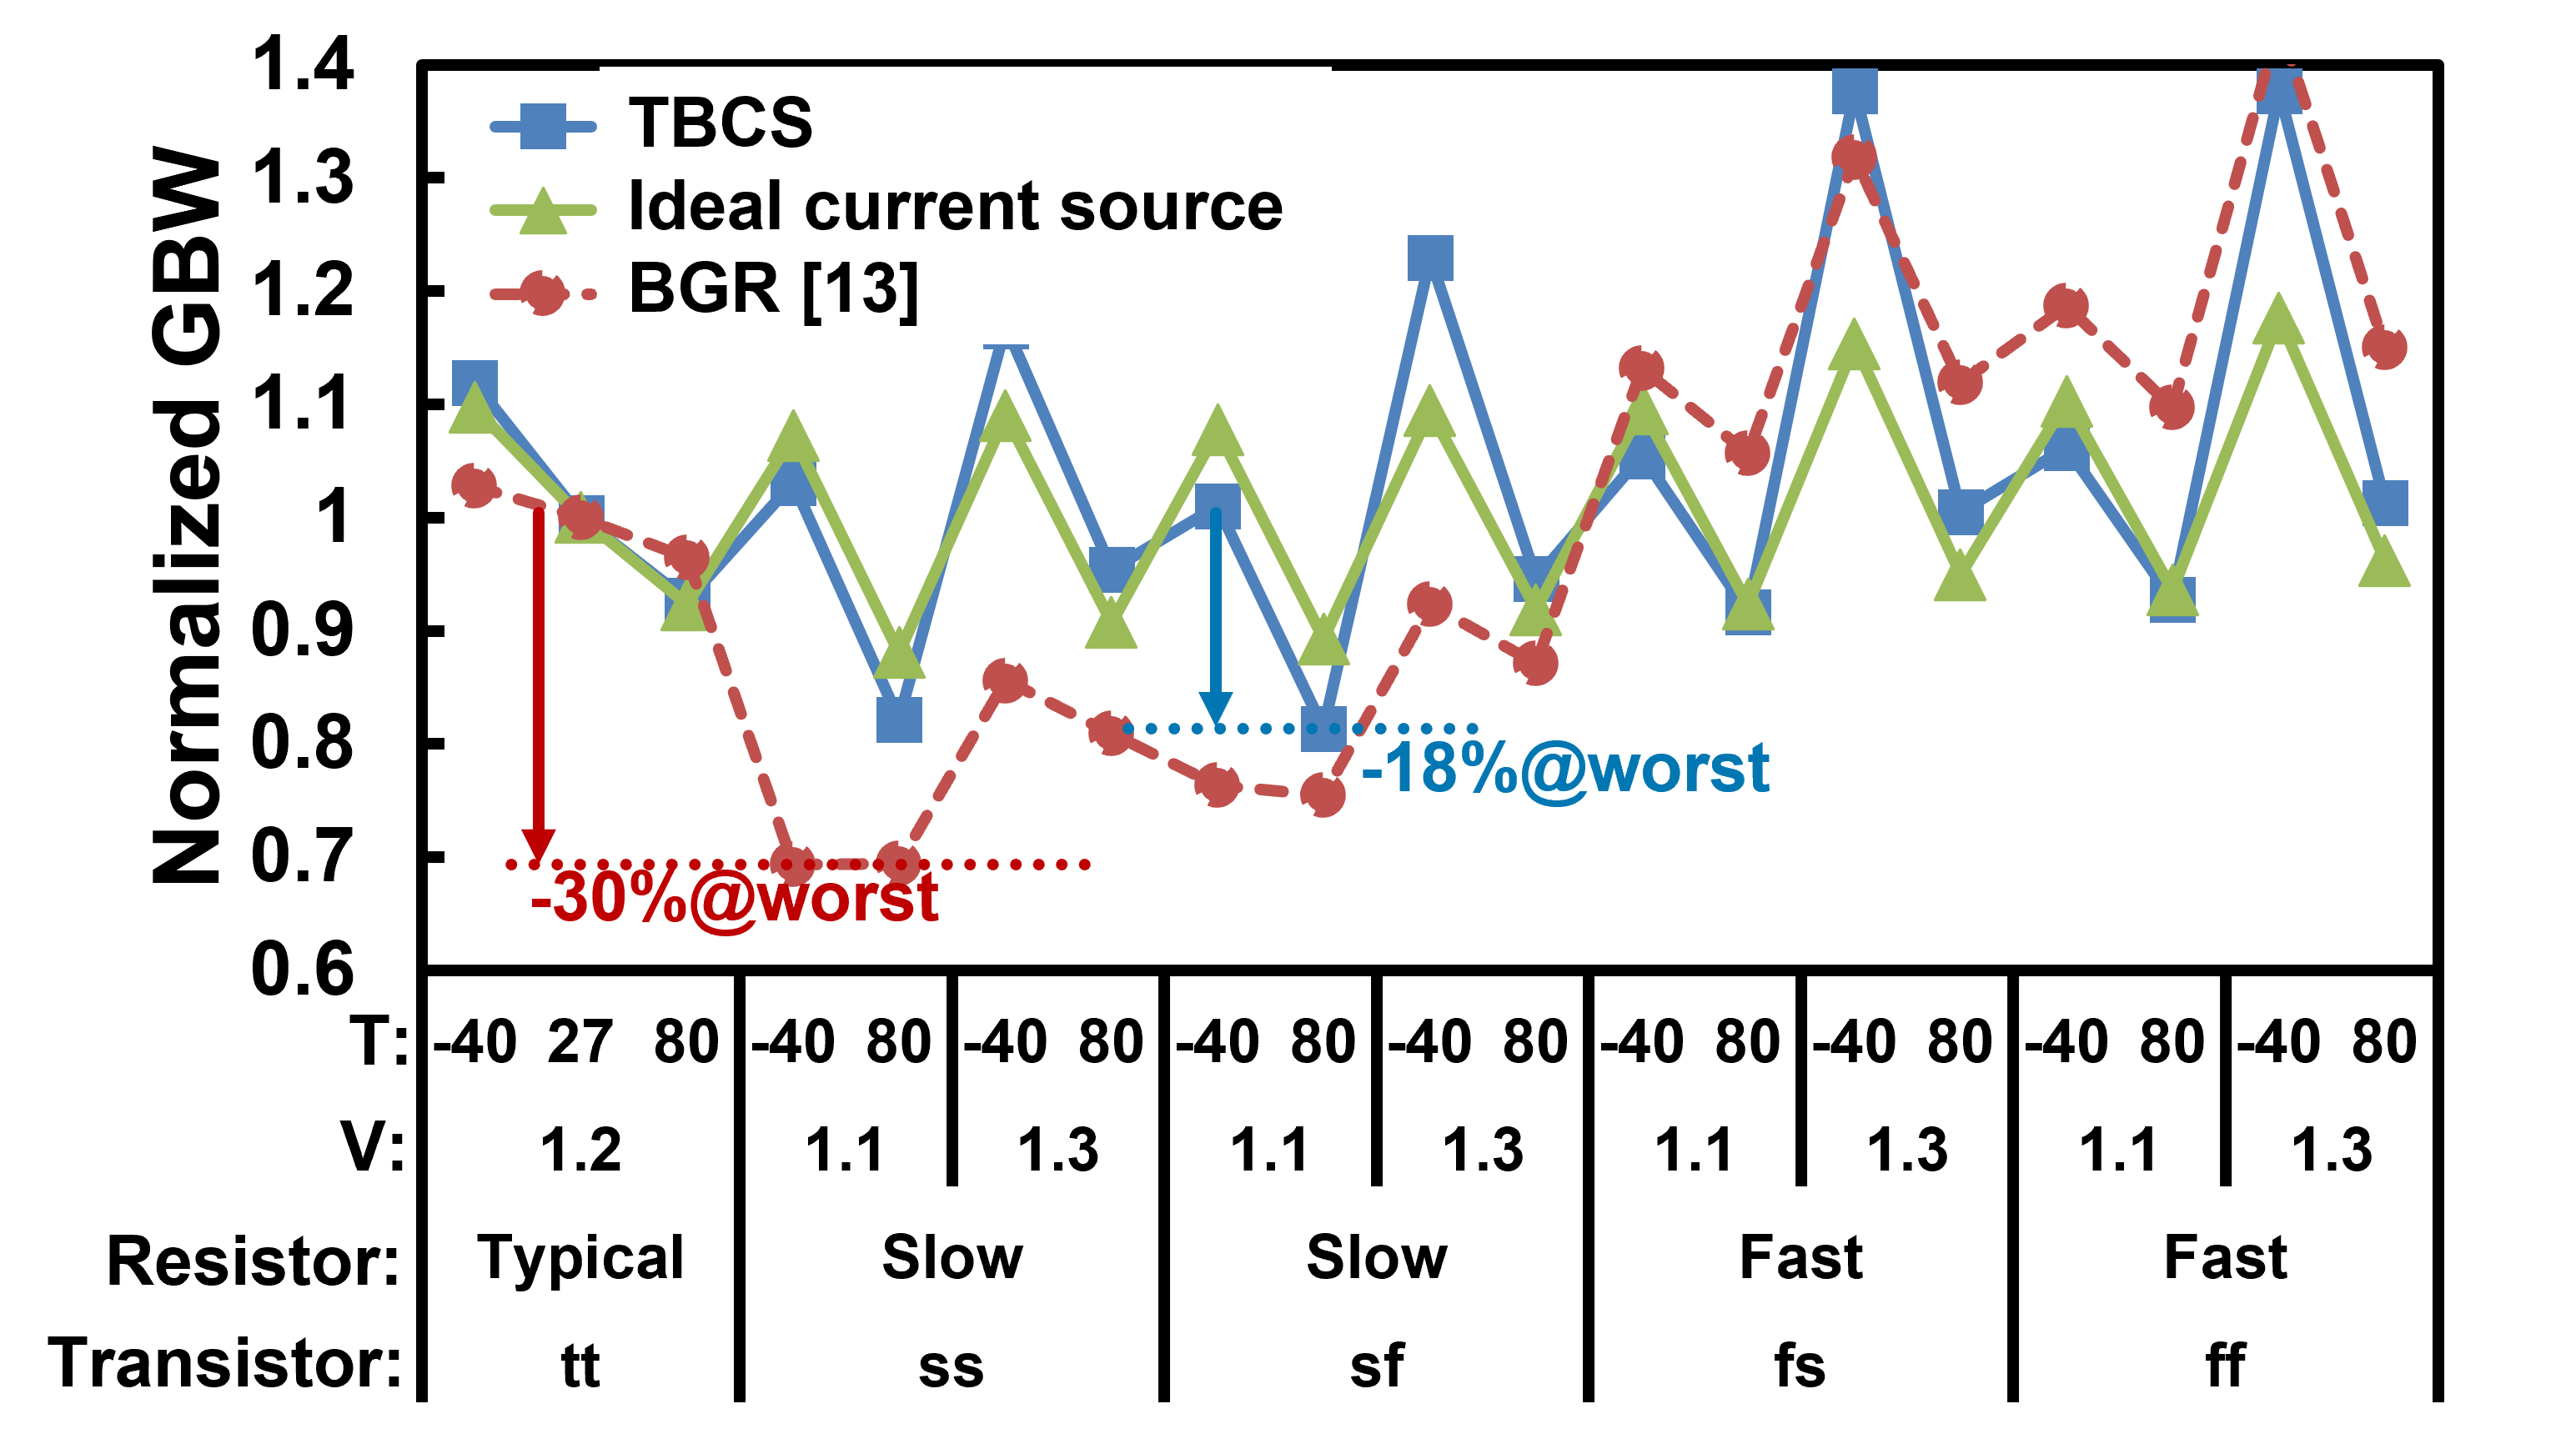
\includegraphics[width=0.5\textwidth]{figs/pvt_gbw.png}
  \caption{(a) 
}
\label{iref_gbw}
\end{figure}


% 試作と方針説明
The prototype TBCS was fabricated with 28nm CMOS and the chip photograph is shown in Fig. \ref{chip}. TBCS occupies a very small area of $46um \times 26um$ (0.0012$mm^2$). Unlike the BGR, TBCS does not require bipolar transistors or amplifiers and can be easily designed in advanced CMOS with low supply voltage. Since bipolar transistors and opamps have poor CMOS scaling characteristics, realizing them in scaled CMOS results in a relatively high cost.

In the prototype chip, the TBCS is integrated in the ADC of ref.\cite{yoshioka201728}. Since the prototype does not have an $I_{ref}$ monitoring pin, it is not possible to directly measure the detailed characteristics of the TBCS. Thus, simulation analysis are mainly reported \footnote{For NDA reasons, all simulation results are reported based on the circuit reimplemented in 65nm CMOS}. On the other hand, switched-capacitor and ADC operation over a wide range of environmental variations was confirmed by measurements, which indirectly suggests that TBCS is functioning in silicon. The SC circuit circuit diagram and the SNDR evaluation results of the ADC are shown in Fig.\ref{scap} and Fig.\ref{sndr}, respectively. The SC circuit employs two-stage amplification: the opamp biased by TBCS performing the coarse amplification and the successive-approximation circuit performs the fine amplification. Sufficient accuracy cannot be obtained if the opamp is not functioning. The ADC achieves a high SNDR (60dB) at a range of -40 to 125$\degC$, indicating that the TBCS and SC circuits are fully-functional.

% 電流源としての性能評価
Firstly, we compare the $I_{ref}$ of BGR current source (BGR ref) as in Fig.\ref{bandgap} and TBCS, respectively. Fig.\ref{iref_pvt_both} shows the simulation results of both current sources under the written PVT variations. The BGR ref with poly-resistors has a large sensitivity to temperature and manufacturing variations, and the min-max current value is more than 30uA. The variance is especially large at SSLTLV conditions, where $I_{ref}$ drops by 40\% compared to typical conditions.
Since this corner condition is where the opamp speed is most severe as well, it is difficult to satisfy the target GBW. In general, the operating current must be enlarged to satisfy the speed at SSLTLV conditions, resulting in a large power overhead.

In addition, the large $I_{ref}$ increase in the FF condition also poses a problem: the increase in $I_{ref}$ requires to increase transistor $V_{gs}$ to compensate. This may narrow down the output range of the opamp under such conditions. To make the opamp characteristics robust, it is desirable that $I_{ref}$ increases in the SS condition and decreases in the FF condition.

一方で図\ref{iref_pvt_both}にTBCSの電流値もプロットした。入力クロック周波数は80MHzであり、その時に電流源は30uA出力するよう設計している。電流値は遅延ロックしたあとの値をプロットしている。BGR refとの違いとしてまずPVTばらつき下でもmin-max電流差が少ない。従来電流源の設計では抵抗値ばらつきによってmin-max差が30uAもあったのに対し、TBCSでは14uAとPVTばらつきを半分程度に削減する。

% GBWのシミュレーション結果
次に図\ref{iref_gbw}にてBGR, ideal, TBCS電流源を用いた際のそれぞれのPVTばらつきにおけるオペアンプGBWシミュレーション結果を報告する。
BGR refはSS条件において電流減少してしまう効果があり理想電流源使用時と比べGBWは大きく減少しワーストコーナーではオペアンプGBWは30\%低下してしまう。このような状況だとオペアンプの設計マージンを拡大しなければならず、回路全体の消費電力は大きく増加してしまう。
一方でTBCSを用いるとPVT適応的な電流を生成する効果もあり、理想電流源とほぼオペアンプGBWは変わらない。ワーストコーナーでもGBW劣化は18\%とBGR refの半分程度に抑えることができ、オペアンプ設計マージンを抑えることができる。

\section{Conclusions}
微細CMOSに好適なスイッチドキャパシタ回路用基準電流源回路であるTime-Based Current Source (TBCS)を提案した。TBCSは入力クロックの時間情報を基準に電流を生成するため抵抗に左右されず、プロセス、温度、電源電圧のばらつきに対しロバストでありバンドギャップ電流源に対し変動を半分に抑える。またTBCSはほぼインバータセルと簡潔なデジタル回路で実現することができ、28nm CMOSにおいて1200um2と非常に小さい面積で実現する。またTBCSのユニークな点として負荷容量のばらつきに応じ生成電流を変動させるが、これはスイッチドキャパシタ回路のオペアンプGBWを補償する特徴を持つ。

\bibliographystyle{IEEEbib}
\bibliography{main}


\begin{IEEEbiography}
[{
\includegraphics[width=1in,height=1.25in,clip,keepaspectratio]{bio/1.jpg}}]{Kentaro Yoshioka}
received his BS, MS, Ph.D degrees from Keio University, Japan. Currently, he is an Assistant Professor at Keio University. He worked with Toshiba during 2014-2021, developing circuitry for WiFi and LiDAR SoCs. During 2017-2018, he had been a visiting scholar at Stanford University, exploring efficient machine learning hardware and algorithms. 

Currently, Dr. Yoshioka serves as a technical program member of Symp. VLSI circuits conference. He was the recipient of ASP-DAC 2013 Special Feature Award, the A-SSCC 2012 Best Design Award, and 1st place winner of Kaggle 2020 Prostate Cancer Grade Assessment (PANDA) Challenge.
\end{IEEEbiography}

\end{document}
